
A hidden layers in neural network consists are layers in between the input layer and the ouput layer. each layer consists of columns of neurons, and are connected to neurons in adjacent layers. The connection between the neurons are called weights, and are represented by a real number value. These weights are individual, meaning that two neurons in the same layer, recieving the same input, can have different weights associated to it. A neuron in a hidden layer, takes as input, all of the attached neurons multiplied by their weight, summed including a fixed bias and passed through an activation function to a scalar-output. this activation function is in our case a lineare rectified unit.\\

\noindent
Presenting this as a function, the sum of the multiplied weights and added bias we define as $y_i$. We then define the connected neurons $x_j$ for $j \in$ \{1,...,N\}, where N is the amount of the connected neurons. We define the associated weights as $w_{ij}$ and added bias as $b_i$. Having the activation function as $\phi()$:

\begin{align}
	y_i &= \sum^N_{j=1} x_jw_{ij} + b_i\\
	a_i &= a(y_i) \\
	a_i &=\left\{ \begin{matrix}
		a_i \geq 0 = a_i \\
		\\
		a_i < 0 = 0
	\end{matrix}
	\right.
\end{align}


\begin{figure}[!ht]
  \centering
  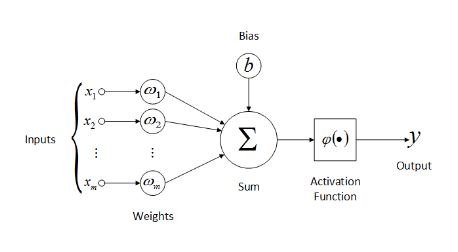
\includegraphics[scale=1.0]{latex/IMGs/neuronFunc.png}
  \caption{Diagram represeinting how a neuron calcutlates its value}\label{Baseline:before}
\end{figure}

\noindent
When training the neural network, the only parameter which is changing is the weights. Since the weight from the neuron(1) is multiplied with the weight connecting to neuron(2), the magnitude of this weight defines how much influence neuron(1) has on neuron(2). Thus, the quality of the model, depends on how good it is at adjusting the weights, and by that learning the model to map input to a nice estimation of a correct output.
